\documentclass[12pt,a4paper]{article}

% Packages
\usepackage[utf8]{inputenc}    % Unicode support
\usepackage{amsmath,amsfonts}  % Math symbols
\usepackage{graphicx}          % Images
\usepackage{hyperref}          % Hyperlinks
\usepackage{geometry}          % Page layout
\usepackage{caption}           % Captions for figures/tables
\usepackage{cite}              % Citations


% Page layout settings
\geometry{
    top=1in,
    bottom=1in,
    left=1in,
    right=1in
}

% Title information
\title{RoboSurgery}
\author{Matteo Nunziante\thanks{matteo.nunziante@studenti.units.it}}
\date{\today}

\begin{document}

% Title
\maketitle

% Abstract
\begin{abstract}

\end{abstract}

% Keywords
\textbf{Keywords:} keyword1, keyword2, keyword3
\newpage


% Table of contents
\tableofcontents 
\newpage

% Introduction
\section{Introduction}
The goal of this project is to simulate a surgical robot for exploring lungs of patients.
% Related Work
\section{Related Work}

% Methodology
\section{Probkem Statement}


% POMDP
\section{POMDP}
Formal description of Partially Observable Markov Decision Process as in \cite{Spaan2012}

Formally, a POMDP is a 7-tuple $(S,A,T,R,\Omega,O,\gamma)$, where: \\
  $S$ is a set of states, \\
  $A$ is a set of actions, \\
  $T$ is a set of conditional transition probabilities between states, \\
  $R: S\times A \rightarrow \mathbb{R}$  is the reward function. \\
  $\Omega$ is a set of observations, \\
  $O$ is a set of conditional observation probabilities, \\
  $\gamma \in [0,1)$ is the discount factor.

\newpage
\section{Mathematical Formulation}
\subsection{State Space}
We are interested in the estimation of the deformaition parameters of an object in a 2D space.
$$s = (\theta)$$

$\theta$ represents the deformation tensor.

\subsection{Action Space}
The action space is the set of all possible actions that the robot can take, 
Forwards, Backwards, Left, Right.
\subsection{Observation Space}
The observation space is the set of all possible observations that the robot can make,
i.e. the presence or absence of an obstacle in its field of view.
\subsection{Bayesian estimation}

rendere il belief indipendente dalla posizione e orientazione del robot, dipenderò unicamente dalla deformazione

$$b(s) = b(theta) * \delta(xyphi = real(xyphi))$$

real(xyphi) = x*
from now on x = xyphi



$$b'_{a,o}(x',\theta') = \eta \cdot \delta(x'=x^*+a) \cdot p(o|x',\theta') \cdot \sum_{x,\theta}p(x',\theta'|x,\theta,a)b(x,\theta)$$
$$ = \eta \cdot \delta(x'=x^*+a) \cdot p(o|x',\theta') \cdot b(x'-a,\theta') $$
$$ = \eta \cdot \delta(x'=x^*+a) \cdot p(o|x',\theta') \cdot \delta (x'-a = x^* )b(\theta') $$
$$ = \eta \cdot \delta(x'=x^*+a) \cdot p(o|x',\theta') \cdot b(\theta') $$
$$ = \eta \cdot \delta(x'=x^*+a) \cdot b'_{a,o}(\theta')$$

dunque a seconda della azione scelta i non zero saranno i 4 x raggiungibili con a

$$p(o|b,a) = \sum_{x,\theta}p(o|x,\theta)b(x.\theta)$$
$$ = \sum_{\theta}p(o|x^*,\theta)b(\theta)$$
% Conclusion
\newpage
\section{Results}
\subsection{MDP Solution}
\subsection{QMDP}

\begin{center}
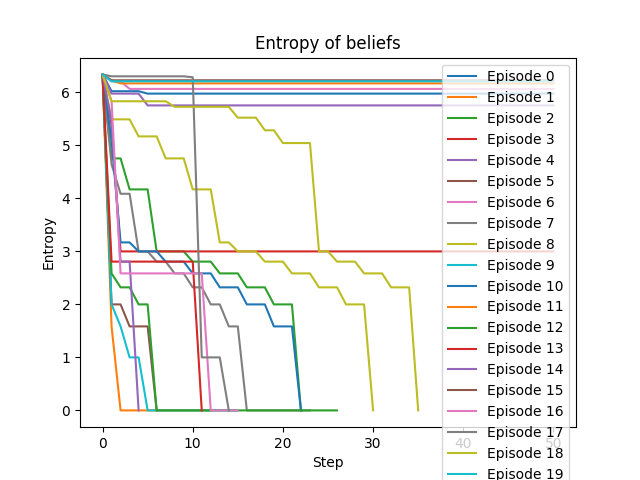
\includegraphics[scale=0.7]{../src/plots/Qentropy_13out20.png}
\end{center}

reaching target 13 out of 20 times.

\subsection{Thompson Sampling}
\begin{center}
  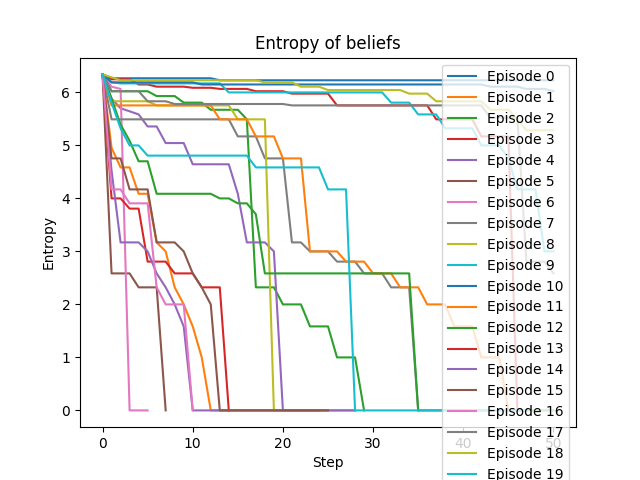
\includegraphics[scale=0.7]{../src/plots/Thompsonentropy_14out20.png}
\end{center}
  
reaching target 14 out of 20 times.

\subsection{Infotaxis}
\begin{center}
  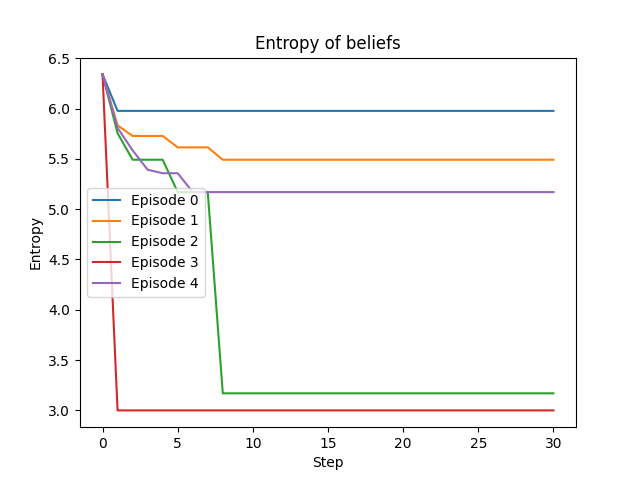
\includegraphics[scale=0.7]{../src/plots/Infotaxisentropy_0out5.png}
\end{center}

reaching target 15 out of 20 times.

\subsection{Information Directed Sampling}
\cite{russo2017learningoptimizeinformationdirectedsampling}

\begin{center}
  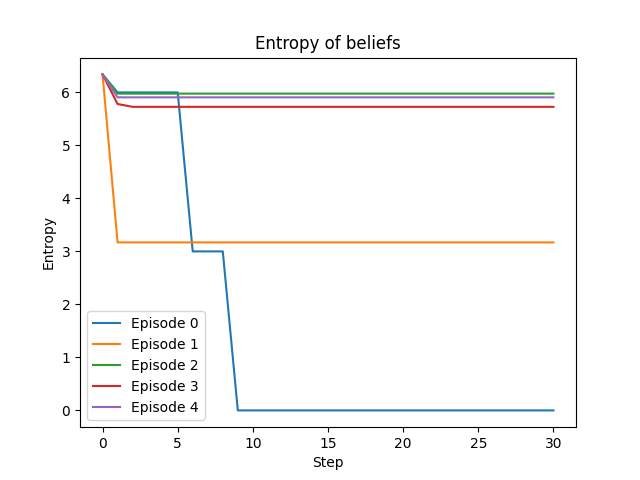
\includegraphics[scale=0.7]{../src/plots/IDSentropy_0out5.png}
\end{center}

reaching target 0 out of 5 times


\subsection{DQN}




% References
\newpage
\bibliographystyle{plain}
\bibliography{ref}


\end{document}
